\documentclass[a4paper]{article} 
\addtolength{\hoffset}{-2.25cm}
\addtolength{\textwidth}{4.5cm}
\addtolength{\voffset}{-3.25cm}
\addtolength{\textheight}{5cm}
\setlength{\parskip}{0pt}
\setlength{\parindent}{0in}

\usepackage[square,sort,comma,numbers]{natbib}
\usepackage{blindtext} % Package to generate dummy text
\usepackage{charter} % Use the Charter font
\usepackage[utf8]{inputenc} % Use UTF-8 encoding
\usepackage{microtype} % Slightly tweak font spacing for aesthetics
\usepackage{amsthm, amsmath, amssymb} % Mathematical typesetting
\usepackage{float} % Improved interface for floating objects
\usepackage{hyperref} % For hyperlinks in the PDF
\usepackage{graphicx, multicol} % Enhanced support for graphics
%\usepackage{xcolor} % Driver-independent color extensions
\usepackage{pseudocode} % Environment for specifying algorithms in a natural way
\usepackage[mmddyy]{datetime} % Uses YEAR-MONTH-DAY format for dates
\usepackage[table,xcdraw]{xcolor}

\usepackage{fancyhdr} % Headers and footers
\pagestyle{fancy} % All pages have headers and footers
\fancyhead{}\renewcommand{\headrulewidth}{0pt} % Blank out the default header
\fancyfoot[L]{} % Custom footer text
\fancyfoot[C]{} % Custom footer text
\fancyfoot[R]{\thepage} % Custom footer text
\newcommand{\note}[1]{\marginpar{\scriptsize \textcolor{red}{#1}}} % Enables comments in red on margin

\DeclareMathOperator*{\argmin}{arg\,min}

%----------------------------------------------------------------------------------------


%-------------------------------
%	TITLE VARIABLES (identify your work!)
%-------------------------------

\newcommand{\yourname}{Jérémie Dentan} % replace YOURNAME with your name
\newcommand{\youremail}{jeremie.dentan@live.com} % replace YOUREMAIL with your email
\newcommand{\assignmentnumber}{3} % replace X with the lab session number

\begin{document}

%-------------------------------
%	TITLE SECTION (do not modify unless you really need to)
%-------------------------------
\fancyhead[C]{}
\hrule \medskip
\begin{minipage}{0.295\textwidth} 
\raggedright
\footnotesize
\yourname \hfill\\
\youremail
\end{minipage}
\begin{minipage}{0.4\textwidth} 
\centering 
\large 
Homework \# \assignmentnumber\\ 
\normalsize 
Convex optimization 2022\\ 
\end{minipage}
\begin{minipage}{0.295\textwidth} 
\raggedleft
\today\hfill\\
\end{minipage}
\medskip\hrule 
\bigskip



%-------------------------------
%	ASSIGNMENT CONTENT (add your responses)
%-------------------------------


\section{Question 1}

This question is a direct consequence of question 2 of homework 2. The dual problem we obtained for (LASSO) is:

$$
\min_v \frac{1}{2}||v||^2_2 + y^Tv
$$

$$
\text{s.t.  } ||X^Tv||_\infty \le \lambda
$$

With the notations of the homework, this is a particular form of (QP) with:

$$
Q = 0.5 I_n \ \ ; \ \
p = y \ \ ; \ \
A = \begin{bmatrix}
    X^T \\
    -X^T \\
\end{bmatrix} \in \mathbb{R}^{2d\timesn} \ \ ; \ \
d = \begin{bmatrix}
    \lambda \\
    \vdots \\
    \lambda
\end{bmatrix} \in \mathbb{R}^{2d}
$$

\section{Question 2}

We want to solve (QP). With the notations of the homework, we first write $(a_1, ... a_M)$ the lines of matrix A:

$$
A = \begin{bmatrix}
    a_0^T \\
    \vdots \\
    a_m^T \\
\end{bmatrix}
$$

Then, by definition, the barrier problem is :

$$
\min_v t(v¨tQv + p^Tv) - \sum_{i=1}^m\log(b_i - a_i^Tv)
$$

Let $f_t(v)$ be the objective function of this minimization problem. For more simplicity, let $g_i(v) = b_i - a_i^Tv$. The gradient is given by:

$$
\nabla f_t(v) = 2tQv + tp + \sum_{i=1}^m \frac{a_i}{g_i(v)}
$$

Let $h_i(v) = \frac{a_i}{g_i(v)}$. The the hessian is given by:

$$
\nabla^2f_t(v) = 2tQ + \sum_{i=1}^m\frac{a_ia_i^T}{g_i(v)^2} = 2tQ + \sum_{i=1}^m h_i(v)h_i(v)^T
$$

Those computations are then used in our implementation of the Newton method. Please refer to scripts in \texttt{/src/centering.py} and \texttt{/src/barrier.py}.

\section{Question 3}

Please refer to our implementation in \texttt{/src/mse.py}. Please refer to \texttt{README.md} for further detail to run the code.

The figure we obtained is presented in figure \ref{fig:muComp}

\begin{figure}[!h]
    \centering
	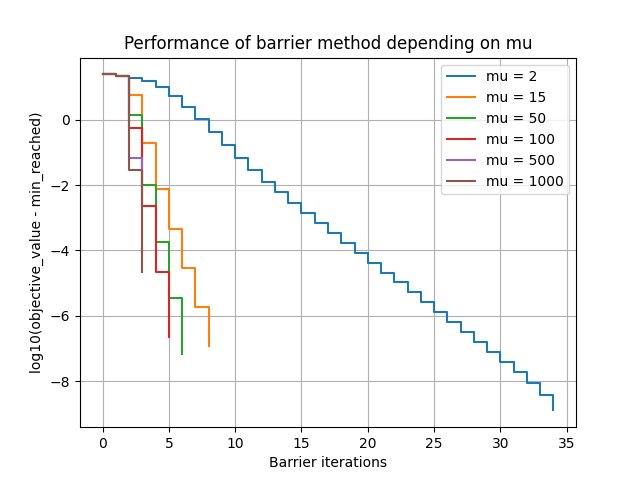
\includegraphics[width=1\textwidth]{figures/mu_performances.png}
	\caption{Performances depending on $\mu$ \label{fig:muComp}}
\end{figure}


%------------------------------------------------

%\bibliographystyle{plain}
%\bibliography{references} % citation records are in the references.bib document

\end{document}
